\documentclass[tikz,border=0pt]{standalone}
\usepackage{amsmath,bm}
\usetikzlibrary{arrows.meta,positioning,calc}
\definecolor{iotfill}{RGB}{240,240,240}\definecolor{iotdraw}{RGB}{120,120,120}
\definecolor{agfill}{RGB}{236,230,250}\definecolor{agdraw}{RGB}{120,90,190}
\definecolor{edfill}{RGB}{230,244,232}\definecolor{eddraw}{RGB}{60,140,80}
\definecolor{clfill}{RGB}{228,238,250}\definecolor{cldraw}{RGB}{50,110,180}
\definecolor{envdraw}{RGB}{110,110,110}\definecolor{arr}{RGB}{50,50,50}
\newcommand{\ttl}{\fontsize{8}{9.5}\selectfont\bfseries}
\newcommand{\bdy}{\fontsize{7}{8.5}\selectfont}
\tikzset{
 box/.style={draw,rounded corners=2pt,line width=0.6pt,align=center,inner sep=2pt,font=\bdy},
 flow/.style={-{Stealth[length=3.6pt,width=3.2pt]},line width=0.7pt,draw=arr},
 badge/.style={circle,fill=black,text=white,inner sep=0pt,minimum size=8pt,font=\fontsize{6}{6}\selectfont\bfseries,text height=1.45ex,text depth=0pt},
 lab/.style={font=\bdy,inner sep=1pt},
}
\newcommand{\bdg}[1]{\tikz[baseline=(b.base)]\node[badge](b){#1};}
\begin{document}
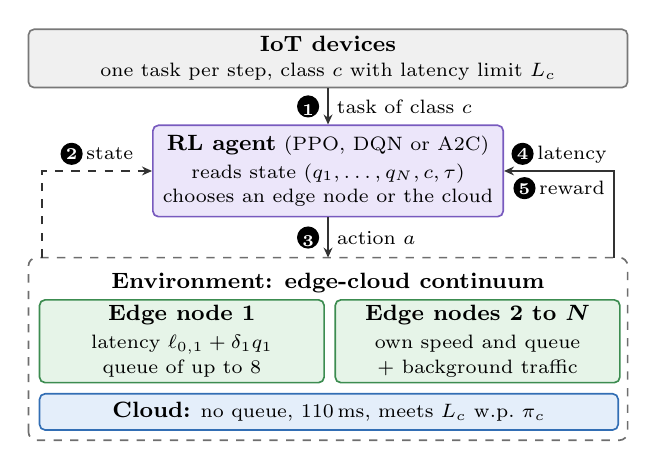
\begin{tikzpicture}
\def\W{7.629}  % = \columnwidth of the journal (216.24pt)
\def\H{5.25}
\useasboundingbox (0,0) rectangle (\W,\H);
% IoT devices
\node[box,fill=iotfill,draw=iotdraw,minimum width=\W cm-0.6pt,minimum height=0.74cm,anchor=north] (iot) at (\W/2,\H-0.01)
 {{\ttl IoT devices}\\[0.5pt]one task per step, class $c$ with latency limit $L_c$};
% RL agent
\node[box,fill=agfill,draw=agdraw,minimum width=4.45cm,minimum height=1.16cm] (ag) at (\W/2,3.43)
 {{\ttl RL agent} (PPO, DQN or A2C)\\[1.5pt]reads state $(q_1,\dots,q_N,c,\tau)$\\[0.5pt]chooses an edge node or the cloud};
% Environment
\def\ET{2.33}
\draw[envdraw,dashed,line width=0.6pt,rounded corners=3pt] (0.01,0.01) rectangle (\W-0.01,\ET);
\coordinate (envtop) at (\W/2,\ET);
\node[font=\ttl,anchor=north] at (\W/2,\ET-0.07) {Environment: edge-cloud continuum};
\def\gap{0.12}\def\mx{0.14}
\pgfmathsetmacro{\bw}{(\W-2*\mx-\gap)/2}
\pgfmathsetmacro{\cw}{\W-2*\mx}
\node[box,fill=clfill,draw=cldraw,minimum width=\cw cm,minimum height=0.46cm,anchor=south west] (cl) at (\mx,0.13)
 {{\ttl Cloud:} no queue, 110\,ms, meets $L_c$ w.p.\ $\pi_c$};
\node[box,fill=edfill,draw=eddraw,minimum width=\bw cm,minimum height=1.04cm,anchor=south west] (e1) at ($(cl.north west)+(0,\gap)$)
 {{\ttl Edge node 1}\\[1.5pt]latency $\ell_{0,1}+\delta_1 q_1$\\[0.5pt]queue of up to 8};
\node[box,fill=edfill,draw=eddraw,minimum width=\bw cm,minimum height=1.04cm,anchor=south west] (e2) at ($(e1.south east)+(\gap,0)$)
 {{\ttl Edge nodes 2 to $\bm{N}$}\\[1.5pt]own speed and queue\\[0.5pt]+ background traffic};
% 1: task
\draw[flow] (iot.south) -- (ag.north) coordinate[midway] (m1);
\node[badge,left=3pt of m1] {1};
\node[lab,right=2pt of m1] {task of class $c$};
% 3: action
\draw[flow] (ag.south) -- (envtop) coordinate[midway] (m3);
\node[badge,left=3pt of m3] {3};
\node[lab,right=2pt of m3] {action $a$};
% 2: state (left, dashed)
\draw[flow,dashed] (0.18,\ET) |- (ag.west) coordinate[pos=0.75] (m2);
\node[lab,above=1pt of m2] {\bdg{2}\,state};
% 4, 5: latency and reward (right)
\draw[flow] (\W-0.18,\ET) |- (ag.east) coordinate[pos=0.75] (m4);
\node[lab,above=1pt of m4] {\bdg{4}\,latency};
\node[lab,below=1pt of m4] {\bdg{5}\,reward};
\end{tikzpicture}
\end{document}
